% Created 2021-12-28 mar 17:43
% Intended LaTeX compiler: pdflatex
\documentclass[conference]{IEEEtran}
\usepackage[utf8]{inputenc}
\usepackage[T1]{fontenc}
\usepackage{graphicx}
\usepackage{longtable}
\usepackage{wrapfig}
\usepackage{rotating}
\usepackage[normalem]{ulem}
\usepackage{amsmath}
\usepackage{amssymb}
\usepackage{capt-of}
\usepackage{hyperref}
\input{~/org/latex/author_TeoCir2_Riedinger.tex}
\input{~/org/latex/ieee.tex}
\date{\today}
\title{Diseño de filtros digitales TIIR basados en el microcontrolador STM32F429ZI}
\hypersetup{
 pdfauthor={},
 pdftitle={Diseño de filtros digitales TIIR basados en el microcontrolador STM32F429ZI},
 pdfkeywords={},
 pdfsubject={},
 pdfcreator={Emacs 27.2 (Org mode 9.6)}, 
 pdflang={Spanish}}
\begin{document}

\maketitle
\tableofcontents


\section{Introducción:}
\label{sec:orgf52369c}

Un filtro es un sistema, que dependiendo de algunos parámetros, realiza un proceso de discriminación de una señal de entrada obteniendo  variaciones en su salida. Los filtros digitales tienen como entrada una señal digital y a su salida tienen otra señal digital, pudiendo haber cambiado en amplitud, frecuencia o fase dependiendo de las características del filtro.

El filtrado digital es parte del procesado de señal digital. Se le da la denominación de digital más por su funcionamiento interno que por su dependencia del tipo de señal a filtrar, así podríamos llamar filtro digital tanto a un filtro que realiza el procesado de señales digitales como a otro que lo haga de señales analógicas.

El filtrado digital consiste en la realización interna de un procesado de datos de entrada. El valor de la muestra de la entrada actual y algunas muestras anteriores (que previamente habían sido almacenadas) son multiplicadas, por unos coeficientes definidos. También podría tomar valores de la salida en instantes pasados y multiplicarlos por otros coeficientes. Finalmente todos los resultados de todas estas multiplicaciones son sumados, dando una salida para el instante actual. Esto implica que internamente tanto la salida como la entrada del filtro serán digitales, por lo que puede ser necesario una conversión analógico‐digital o digital‐analógico para uso de filtros digitales en señales analógicas.

Los filtros digitales se usan frecuentemente para tratamiento digital de la imagen o para tratamiento del sonido digital.

\subsection{Tipos de filtros:}
\label{sec:org223e233}

Hay varios tipos de filtros así como distintas clasificaciones para estos filtros:

\begin{itemize}
\item De acuerdo con la parte del espectro que dejan pasar y atenúan hay:

\begin{itemize}
\item Filtros pasa alto.
\item Filtros pasa bajo.
\item Filtros pasa banda.
\begin{itemize}
\item Banda eliminada.
\item Multibanda.
\item Pasa todo.
\item Resonador.
\item Oscilador.
\item Filtro peine (Comb filter).
\item Filtro ranura o filtro rechaza banda (Notch filter).
\end{itemize}
\end{itemize}

\item De acuerdo con su orden:

\begin{itemize}
\item Primer orden.
\item Segundo orden o superior.
\end{itemize}

\item De acuerdo con el tipo de respuesta ante la entrada unitaria:

\begin{itemize}
\item FIR (Respuesta Finita al Impulso o \emph{Finite Impulse Response}).
\item IIR (Respuesta Infinita al Impulso o \emph{Infinite Impulse Response}).
\item TIIR (Respuesta Infinita Truncada al Impulso o \emph{Truncated Infinite Impulse Response}).
\end{itemize}

\item De acuerdo con la estructura con que se implementa:

\begin{itemize}
\item Directa.
\item Transpuesta.
\item Cascada.
\item Fase lineal.
\item Laticce.
\end{itemize}
\end{itemize}

\subsection{Comparación entre los distintos tipos de filtros:}
\label{sec:org91d9bb1}

Los filtros IIR son ampliamente utilizados debido a su bajo costo computacional. Los filtros FIR, en cambio, permiten la posibilidad de implementar filtros lineales digitales con un retraso de grupo constante para todas las frecuencias. La contrapartida es que, para alcanzar funciones de transferencia de magnitud similar, los filtros FIR requieren un orden mucho mayor que su contraparte IIR. Por ejemplo,  La contrapartida es que, para alcanzar funciones de transfer    de magnitud similar, los filtros FIR requieren un orden mucho mayor que su contraparte IIR. Por ejemplo, un filtro general FIR de orden \(N\) requieren \(N+1\) múltiplos y \(N\) sumandos.

En ciertos casos, sin embargo, es posible diseñar filtros FIR con costo computacional comparable al de los filtros IIR mientras se mantienen las ventajas que proporcionan los filtros FIR. Este tipo de filtros FIR puede ser implementado de forma eficiente mediante secuencias truncadas de bajo orden de filtros IIR. A este tipo de filtros se los conoce como filtro TIIR.

\subsection{Expresión general de un filtro digital:}
\label{sec:org2223ed3}

En muchas aplicaciones del procesado de señales es necesario diseñar dispositivos o algoritmos que realicen operaciones sobre las señales y que los englobaremos bajo la denominación genérica de sistemas.

Un sistema opera sobre una señal de entrada o excitación según una regla preestablecida, para generar otra señal llamada salida o respuesta del sistema a la  excitación propuesta y que puede simbolizarse:

\begin{equation}
    y[n] = T(x[n])
\end{equation}

donde \(T\) simboliza la transformación, operador o procesado realizado por el sistema sobre la señal \(x\) para producir la señal \(y\) (ver Fig. \ref{fig:esquemaFiltro}). Una de las motivaciones más fuertes para el desarrollo de herramientas generales para el análisis y diseño de sistemas es que proviniendo a menudo de aplicaciones muy diferentes tienen descripciones matemáticas similares.

\begin{figure}[htbp]
\centering
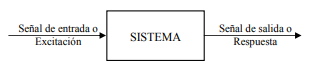
\includegraphics[width=.9\linewidth]{../images/esquemaFiltro.png}
\caption{\label{fig:esquemaFiltro}Esquema de sistema, señal de entrada y respuesta o salida del sistema}
\end{figure}

Existen varias maneras de representar un sistema, ya que muchos sistemas reales están construidos como interconexiones de varios subsistemas, tal como se grafica en la Fig. \ref{fig:interconexionSistema}.

\begin{figure}[htbp]
\centering
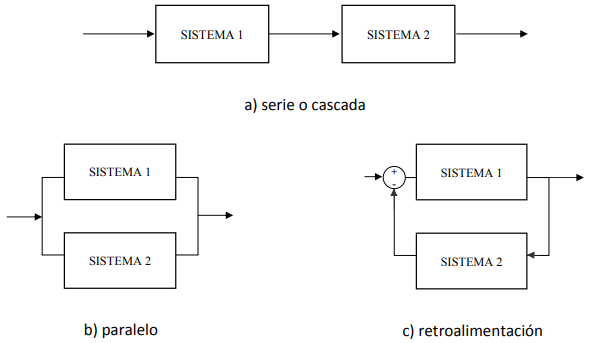
\includegraphics[width=.9\linewidth]{../images/interconexionSistema.png}
\caption{\label{fig:interconexionSistema}Interconexión de sistemas}
\end{figure}

Existen dos métodos básicos para el análisis del comportamiento o respuesta de un sistema lineal a una determinada entrada. Un primer camino se basa en obtener la solución de la ecuación entrada‐salida del sistema que en general tiene la forma de las ecuaciones en diferencias lineales a coeficientes constantes \(a_{m}\), \(b_k\):

\begin{equation}
    \sum_{m=0}^{N_a - 1}{a_m y[n-m]} = \sum_{k=0}^{N_b - 1}{b_k x[n-k]}
    \label{eq:defFiltro}
\end{equation}

siendo \(N_a\) y \(N_b\) los órdenes máximos de las diferencias en la ecuación correspondiente a la entrada y a la saldia del sistema.

El segundo método para el análisis del comportamiento del sistema reside en la aplicación del principio de superposición y consiste en descomponer la señal de entrada en una suma pesada de señales elementales las cuales se escogen de manera que sea conocida la respuesta del sistema a las mismas. Siguiendo esta línea, una señal a tiempo discreto puede visualizarse como una secuencia pesada de impulsos unitarios:

\begin{equation}
    x[n] = \sum_{k=-\infty}^{\infty}{x[k] \cdot \delta [n - k] }
\end{equation}

Aplicando la propiedad de superposición de los SLIT (Sistemas Lineales e Invariantes en el Tiempo) (Oppenheim y Willsky, 1983), se puede determinar la salida del sistema ante una cierta entrada de la siguiente manera:

\begin{equation}
    y[n] = \sum_{k=-\infty}^{\infty}{x[k] \cdot h[n-k]}
\end{equation}

siendo \(h[n]\) la respuesta o salida del sistema ante una entrada equivalente a un impulso unitario \(\delta [n]\) denominada \emph{respuesta al impulso del sistema}. El segundo miembro de la expresión representa el producto de convolución de la señal de entrada \(x[n]\) y la respuesta al impulso del sistema \(h[n]\); esto es:

\begin{equation}
    y[n] = x[n] * h[n] = h[n] * x[n]
\end{equation}

Tanto en el caso continuo como en el caso discreto, la respuesta al impulso del sistema LTI presenta las siguientes propiedades:

\begin{itemize}
\item Sin memoria: \(h[n]=0\) para \(n \neq 0\).
\item Causal: \(h[n]=0\) para \(n<0\).
\item Invertible: dado \(h[n]\: \exists \:h'[n]\::\:h[n]*h'[n]=\delta[n]\).
\item Estable: \(\sum_{k=-\infty}^{\infty}{|h[n]|<\infty}\)
\end{itemize}

Existen otras formas de representar un filtro, todas estas equivalentes a la respuesta al impulso unitario de sistema SLIT, sin embargo muchas veces conviene más una u otra representación. En el caso aplicar la transformada Z, a la \ref{eq:defFiltro} se obtiene la función de transferencia del sistema (Oppenheim y Willsky, 1983; Proakis y Manolakis; 1996; Oppenheim y Schafer, 1999):

\begin{equation}
    H(z) = \frac{\sum_{k=0}^{N_b-1}{b_k z^{-k}}}{\sum_{m=0}^{N_a-1}{a_m z^{-m}}}
    \label{eq:6}
\end{equation}

donde \(z=A\exp(j\Omega)\) es la variable compleja en forma polar. Particularmente si el modulo \(A=1\), la expresión de la Ec. \ref{eq:6} se reduce a la respuesta en recuencia del sistema a través de la transformada de Fourier a tiempo discreto (Oppenheim y Willsky, 1983; Proakis y Manolakis; 1996; Oppenheim y Schafer, 1999):

\begin{equation}
    y[n] = \sum_{k=0}^{N_b-1}{b_k x[n-k]} - \sum_{m=1}^{N_a-1}{a_m y[n-m]}
\end{equation}

donde los coeficientes \(a_m\) y \(b_k\) son los coeficientes que definen el filtro, por lo tanto el diseño consiste en calcularlos. Como regla general se suele dejar el término \(a_0=1\).
\subsection{Definición de filtros FIR e IIR:}
\label{sec:org0e6a2c2}

Un filtro FIR causal de orden \(N\) convencional se puede representar según:

\begin{equation}
    y[n] = \sum_{k=0}^{N}{h_k x[n-k]}
\end{equation}

Donde la función de transferencia tiene la siguiente forma:

\begin{equation}
    H_{FIR}(z) = h_0 + h_1 z^{-1} + \ldots + h_N z^{-N} = z^{-N} C(z)
\end{equation}

Y se define a \(C(z)\) como el polinomio de orden \(N\) formado por los coeficientes \(h_k\).

En cambio, un filtro IIR causal de orden \(P\) tiene la relación:

\begin{equation}
    y[n] = - \sum_{k=1}^{P}{a_k - y[n-k]} + \sum_{l=0}^{P}{b_l x[n-l]}
\end{equation}

Con la función transferencia correspondiente es:

\begin{equation}
    H_{IIR}(z) = \frac{b_0 + b_1 z^{-1} + \ldots + b_P z^{-P}}{1 + a_1 z^{-1} + \ldots + a_P z^{-P}} = \frac{B(z)}{A(z)}
    \label{eq:6}
\end{equation}

Por tanto, \(A(z)\) y \(B(z)\) serán:

\begin{equation}
    A(z) = z^{P} + a_1 z^{P-1} + \ldots + a_P
    \label{eq:8}
\end{equation}

\begin{equation}
    B(z) = b_0 z^P + b_1 z^{P-1} + \ldots + b_P
    \label{eq:9}
\end{equation}

Y pueden ser asumidos como los polinomios de grado \(P\) en \(z\).

El retardo de grupo se define como:

\begin{equation}
    \tau_d(\omega) = - \frac{d \: \arg\{H(e^{j\omega)}\}}{d\omega}
\end{equation}

El retardo de grupo a frecuencia normalizada \(\omega=\nicefrac{2 \pi f}{f_s}\); donde \(f_s\) es la frecuencia de muestreo; es el número de muestras con retraso experiezadas por la amplitud de la envolvente de banda ancha centrada en \(\omega\).

Un filtro de fase linear es aquel cuya respuesta en fase a una determinada frecuencia es una función lineal de la frecuencia; esto es, \(\arg \{H(e^{j\omega})\}=K1\omega + K2\) para constantes \(K1\) y \(K2\). A partir de esta propiedad, se nota inmediatamente que el retardo de grupo es constante a todas las frecuencias. Filtro con una respuesta en fase lineal son usualmente los buscados, debido a que no poseen distorsión temporal dependiente de la frecuencia. Un filtro IIR con polos distintos de cero puede tener una fase lineal. Sin embargo, un filtro FIR con coeficiente \(h_0,\ldots , h_N\) tiene fase lineal si existe un \(\varphi\) tal que para todo \(k \in \{0,\ldots , N\}\):

\begin{equation}
    h_{N-k} = e^{j\varphi} h^{*}_k
    \label{eq:11}
\end{equation}

Esto es, si los coeficientes invertidos son conjugados complejos de la próxima secuencia sumados a una constante de cambio de fase, el retardo de grupo será entonces:

\begin{equation}
    \tau_d (f) = \frac{N}{2}
\end{equation}
\section{Filtros IIR truncados (TIIR):}
\label{sec:org83babb5}

Considere un filtro FIR con una secuencia geométricamente truncada \(h_0,h_0p,\ldots , h_0 p^N\) como respuesta al impulso. Este filtro tiene la misma respuesta al impulso para los primeros \(N+1\) términos que un filtro IIR de un solo polo con función de transferencia

\begin{equation}
    H_{IIR}(z) = \frac{h_0}{1- p z^{-1}}
\end{equation}

Si se substrae la "cola" de la respuesta al impulso, se obtiene:

\begin{equation}
    H_{FIR} = h_0 + h_0 p z^{-1} + \ldots + h_0 p^N z^{-N}
\end{equation}

\begin{equation}
    H_{FIR} = h_0 \frac{p^{N-1} z^{-(N+1)}}{1 - p z^{-1}}
    \label{eq:15}
\end{equation}

La recursión en el dominio del tiempo para este filtro estará dada como:

\begin{equation}
    y[n] = \sum_{k=0}^{N}{h_0 p^k x[n-k]}
    \label{eq:16}
\end{equation}

\begin{equation}
   y[n] = p y[n-1] + h_0 \{x[n] - p^{N+1} x[n - (N+1)]\}
   \label{eq:17}
\end{equation}

Se nota que la primer formulación (Ec. \ref{eq:16}) requiere \(N+1\) múltiplos y \(N\) sumandos para ser implementada de forma directa; mientras que la segunda ecuación (Ec. \ref{eq:17}) requiere de solo tres múltiplos y dos sumandos, independientemente de \(N\). Por tanto, se ve que, si se puede representar un FIR como una secuencia exponencial truncada, se encontraría una forma reducida de computar el filtro. Notar que el término \(x[n - (N+1)]\) en la Ec. \ref{eq:17} todavía requiere un retardo para ser mantenido; y por tanto, no hay un reducción en cuanto a almacenamiento.

Existe una cancelación de polo-cero en la representación dada en la Ec. \ref{eq:15}. Si \(|p|<1\) no hay problemas, ya que el sistema será inherentemente estable. Si \(|p|>1\), sin embargo, entonces existe un problema potencial debido al "modo oculto".

La idea de esta sección funciona solo para casos en los que la multiplicidad de cada polo es uno; tal que cada modo exhiba un decaimiento exponencial simple.
\subsection{Extensión a secuencias TIIR de alto orden:}
\label{sec:org778e49b}

Se puede extender la idea ilustrada en la sección anterior para el caso de un polo simple con el objetivo de computar secuencias TIIR de cualquier denominador de \(H(z)\). El procedimiento general es el de encontrar una la "cola" la función transferencia IIR:

\begin{equation}
    H_{IIR}'(z) = h_0' z^{-1} + h_1' z^{-2} + \ldots = h_{N+1} z^{-1} + h_{N+2} z^{-2} + \ldots
\end{equation}

cuya respuesta al impulso, excepto por un cambio temporal de \(N\) pasos, es igual a la "cola" de la función transferencia \(H_{IIR}(z)\), la cual se pretende truncar luego del paso \(N\).

Entonces, multiplicando \(H_{IIR}(z)\) por \(z^N\) se obtiene:

\begin{align}
    z^N H_{IIR} (z) =& h_0 z^N + \ldots + h_{N-1}z + h_N + h_{N+1} z^{-1} + \ldots \\
    =& C(z) + H_{IIR}'(z) \\
    =& \frac{z^N B(z)}{A(z)} \\
    =& C(z) + \frac{B'(z)}{A(z)}
\end{align}

donde \(O[B'(z)] < O[A(z)] = P\). Se puede asumir que \(O[B'(z)]=P-1\). \(B'(z)\) es única y se puede obtener al realizar la división sintética de \(z^N B(z)\) por \(A(z)\) y encontrar el sobrante.

Una vez obtenida \(B'(z)\), se tiene que \(H_{IIR}' = \nicefrac{B'(z)}{A(z)}\), y se puede escribir:

\begin{equation}
    H_{FIR}(z) = H_{IIR}(z) - z^{-N} H_{IIR}'(z) = \frac{B(z)-z^{-N}B'(z)}{A(z)}
\end{equation}

El sistema correspondiente será entonces:

\begin{equation}
\begin{split}
    y[n] =& - \sum_{k=1}^{P}{a_k y[n-k]} + \sum_{l=0}^{P}{b_l x[n-l]}-\\
   & - \sum_{m=0}^{P-1}{b_m ' x[n-m-(N+1)]}
\end{split}
    \label{eq:25}
\end{equation}

El hecho de que los denominadores de las funciones transferencia \(H_{IIR}(z)\) y \(H_{IIR}'(z)\) son los mismos permite un menor costo computacional debido al hecho que el IIR original y la $\backslash$"cola$\backslash$" IIR dinámica son las mismas y no se necesita realizar procedimientos duplicados. El costo computacional de este sistema IIR de orden \(P\) es de \(3P+1\) multiplicandos y \(3P-2\) sumandos, independiente de \(N\). Así, una ganancia computacional con esta clase de filtros FIR es conseguida si \(N>3P\).

El costo de almacenamiento para este filtro son \(P\) muestras de salida para la realimentación dinámica IIR, \(N\) muestras de entrada para el filtro FIR, y un adicional de \(P\) muestras de entrada para la cancelación de la $\backslash$"cola$\backslash$"; significando \(N+P\) muestras de entradas con retraso, de las cuales solo las últimas \(P\) son utilizadas, y \(P\) muestras de salida con retraso. Así, el algoritmo FIR requiere \(2P\) más de almacenamiento que una implementación FIR directa.
\subsection{Otras arquitecutras:}
\label{sec:org30ea55d}

La implementación directa especificada según la Ec. \ref{eq:25} puede ser no deseada por varias razones. Por ejemplo, uno puede optar por utilizar una estructura factorizada tal como la forma bicuadrática cascada o la forma de fracciones paralelas parciales. Esta última está dada como:

\begin{equation}
    H(z) = \sum_{k=1}^{N_p}{\sum_{l=1}^{M_k}{\frac{C_{k,l}}{(1-p_k z^{-1})^l}}}
    \label{eq:26}
\end{equation}

donde \(N_p\) es el número de polos distintos, y \(M_k\) es la multiplicidad del polo número \(k\). El término \((k,l)\) es la expansión por fracciones parciales correspondiente al filtro con respuesta al impulso

\begin{equation}
    h_{k,l}[n] = C_{k,l}
    \left( \begin{array}
        nn+l-1\\
        n-1\\
    \end{array} \right)
    p_{k}^{n}
\end{equation}

Para formar el filtro TIIR, una cola del filtro IIR es derivada por cada fracción parcial utilizando división sintética como se demostró en la sección anterior. Cada respuesta TIIR es calculada de forma separada, y los resultados son sumados para formar la respuesta completa. La factorización no debe ser necesariamente completa como se muestra en la Ec. \ref{eq:26}. Es posible optar por un nivel intermedio de factorización, dejando algunos factores juntos y otros separados. Por ejemplo, se puede optar por agrupar los pares conjugados complejos para evitar aritmética compleja. Alternativamente, se puede dejar los terminos con los mismos polos juntos, según:

\begin{equation}
    H(z) = \sum_{k=1}^{N_p}{\frac{B_k(z)}{(z-p_k)^{M_k}}}
\end{equation}

ya que para cacular la cola de la respuesta IIR para cada término de orden \(n\) se necesita un polinomio de orden \(n-1\) en el numerador de todas formas. La respuesta al impulso de  cada fracción parcial \(k\) en este caso es:

\begin{equation}
    h_{k}[n] = \sum_{l=0}^{M_k}{b_{k,l}}
    \left( \begin{array}
        nn+l+M_k-1\\
        M_k-1\\
    \end{array} \right)
    p_{k}^{n-l}
\end{equation}

donde \(b_{k,l}=0,\ldots ,M_k\) son los coeficientes de \(B_k(z)\).

Otro ejemplo es agrupar a los factores estables juntos; esto es, aquellos con polos \(p_k\) tales que \(|p_k|<1\), e implemetar de forma separada polos inestables para los cuales \(|p_k|>1\).
\section{Filtros FFIR (\emph{Fast} FIR) de fase lineal:}
\label{sec:org227ae0c}

La implementación de filtros como sistemas TIIR no tendría mucho sentido a menos que exista una ventaja que no sea posible con filtros IIR no-truncados. Esta ventaja radica en la posibilidad de realizar filtros de fase-lineal exacte. Se presentarán dos estrategias básicas para el diseño basado en filtros TIIR.

\subsection{Método de diseño por factorización aditiva:}
\label{sec:org3c5a8a3}

Se vió que un filtro FIR tendrá fase linear si se cumple la Ec. \ref{eq:11}. Es posible mantener dicha relación utilizando filtros TIIR. Si \(H_{FIR}^{+}\) es una función transferencia TIIR tal que:

\begin{equation}
    H_{FIR}^{+}(z) = \sum_{k=0}^{N}{h_{k}^{ +}z^{-k}} = \frac{B^{ +}(z)-z^{-N}B^{ +}'(z)}{A^{ + }(z)}
\label{eq:42}
\end{equation}

Formando la función transferencia de tiempo-contrario truncada:

\begin{align}
    H_{FIR}^{-}(z) =& \sum_{k=0}^{N}{h_{k}^{-}z^{-k}} \\
                   =& \sum_{k=0}^{N}{h_{k}^{+*} z^{k-N}} \\
                   =& z^{-N} \left[ H_{FIR}^{ +} \left( \frac{1}{z^{*}} \right) \right] ^{*} \\
                   =& \frac{z^{-N} \left[ B^{ +} \left( \frac{1}{z^{*}} \right) - B^{ +}' \left( \frac{1}{z^{*}} \right)   \right] ^{*}}{\left[ A^{ + } \left( \frac{1}{z^{*}} \right) \right] ^{*}} \\
                   =& \frac{-z B^{-}' (z) + z^{-N} B^{-}(z)}{A^{-}(z)}
\label{eq:47}
\end{align}

donde los superíndices \(+\) y \(-\) denotan 'adelante' y filtro 'reverso-conjugado' respectivamente; y el superíndice \(*\) denota conjugación compleja. De esta forma, comparando con las Ec. \ref{eq:8} y \ref{eq:9} se tiene:

\begin{equation}
    A^{-}(z) = 1 + a^{*}_1 z + \ldots + a^{*}_P z^P
\end{equation}

\begin{equation}
    B^{-}(z) = b_0 + b^{*}_1 z + \ldots + b^{*}_P z^P
\end{equation}

Entonces:

\begin{equation}
    B^{-}'(z) = b_0^{*}' + b_1^{*}' z + \ldots + b_{P_1}^{*}' z^{P-1}
\end{equation}

Se asume que \(B^{+}(z)\) y \(B^{-}'(z)\) tienen ordenes \(P\) y \(P-1\) respectivamente. Si se asume que \(H_{FIR}^{ +}(z)\) es un filtro TIIR estable, entonces \(H_{FIR}^{-}(z)\) es un filtro TIIR inestable cuyos modos escondidos son conjugados recíprocos de los de \(H_{FIR}^{ +}(z)\).

Utilizando un cambio de tiempo arbitrario \(M \geq 0\) y cambio de fase \(\varphi\), se define el filtro:

\begin{align}
    H_{LPFIR}(z) =& H_{FIR}^{ + } (z) + e^{j\varphi} z^{-M} H_{FIR}^{-}(z) \\
                 =& \sum_{k=0}^{N}{h_k^{ + } z^{-k}} + e^{j \varphi} \sum_{k=0}^{N}{h_k^{+*} z^{k-N-M}}
\end{align}

Se nota que este nuevo filtro FIR de longitud \(M+N+1\) es invariante con respecto al orden reverso, conjugando los coeficientes, y multiplicando por un factor de fase \(e^{j\varphi}\). De esta forma, se cumple la Ec. \ref{eq:11}; y así, \(H_{LPFIR}(z)\) es un filtro FIR de fase lineal. Se puede ver la propiedad de fase lineal de forma más directa al notar primero que en el círculo unidad

\begin{equation}
    H_{FIR}^{-}(e^{j\omega}) = e^{-jN\omega} \left[ H_{FIR}^{ + } \left( e^{j\omega} \right ) \right]^{*}
\label{eq:53}
\end{equation}

tal que

\begin{align}
    H_{LPFIR}(e^{j\omega}) =& H_{FIR}^{+}\left( e^{j\omega} \right) + e^{j\varphi} e^{-jM\omega} H_{FIR}^{-} \left( e^{j\omega} \right) \\
                           =& e^{-j[(N + M)\omega + \varphi]/2} H_{FIR}^{ + } \left( e^{j\omega} \right)
\end{align}

por lo que el retardo de grupo resulta en:

\begin{equation}
    \tau_d = \frac{M+N}{2}
\end{equation}

Es relativamente complicado diseñar un FFIR para un determinado set de especificaciones utilizando el método de factorización aditiva debido a que no es intuitivamente obvio como controlar la magnitud \(H_{LPFIR}\left( e^{j\omega} \right)\). Sin embargo, para determinadas respuestas al impulso que están bien caracterizadas, ésta técnica provee una herramienta útil para el diseño de filtros FFIR.
\subsection{Método de diseño por magnitud al cuadrado:}
\label{sec:org397bdd3}

El siguiente método es tal vez de mayor utilidad para el diseño de filtros FFIR en aplicaciones de procesamiento de señal. Se comienza eligiendo una función transferencia no-negativa y real \(H^2(z)>0\) para la cual existe una función transferencia estable \(H(z)\) tal que:

\begin{align}
    H^2 \left( e^{j\omega} \right) =& |H \left( e^{j\omega} \right)|^2\\
                     =& H \left( e^{j\omega} \right) * H \left( e^{j\omega} \right)
\label{eq:57}
\end{align}

y con polinomios \(A^{ + }(z)\) y \(B^{ + }(z)\) tales que:

\begin{align}
    H(z) =& \sum_{k=0}^{\infty}{h_k z^{-k}}\\
         =& \frac{B^{ + }(z)}{A^{ + }(z)}
\end{align}

Si los coeficientes de \(A^{ + }(z)\) y \(B^{ + }(z)\) son reales, entonces la Ec. \ref{eq:57} indica que:

\begin{equation}
    H^2 \left( e^{j\omega} \right) = H \left( e^{j\omega} \right) H \left( e^{-j\omega} \right)
\end{equation}

Formando la función transferencia TIIR

\begin{align}
    H_{FIR}^{ + }(z) =& \sum_{k=0}^{N}{h_k z^{-k}}\\
                     =& \frac{B^{ + }(z) - z^{-N} B^{ + }'(z)}{A^{ + }(z)}
\label{eq:60}
\end{align}

al igual que se hizo en la Ec. \ref{eq:42}. Similarmente, se forma \(H_{FIR}^{-}(z)\) al igual que en la Ec. \ref{eq:47}; y, en vistas de la Ec. \ref{eq:53} se ve que el filtro

\begin{equation}
    H^2_{FIR}(z) = H_{FIR}^{ + }(z) H_{FIR}^{ - }(z)
\end{equation}

tiene la propiedad de

\begin{equation}
    H_{FIR}^{ 2 }\left( e^{j\omega} \right) = e^{-jN\omega} | H_{FIR}^{ +}\left( e^{j\omega} \right) |
\end{equation}

y que obviamente es un filtro de fase lineal con retardo de grupo igual a:

\begin{equation}
    \tau_d = N
\end{equation}

Este filtro puede ser implementado como una cascada de \(H_{FIR}^{ +}(z)\) y \(H_{FIR}^{ -}(z)\), que a su vez pueden ser implementadas según la Ec. \ref{eq:25}.

La relación entre \(H_{FIR}^{2}(z)\) y \(H^2(z)\) se puede ver considerando la convolución cíclica en la Ec. \ref{eq:6}:

\begin{equation}
    H_{FIR}^{ + } \left( e^{j\omega} \right) = \frac{1}{2\pi} \int_0^{2\pi}{H \left( e^{j\theta} \right) W_N \left[ e^{j(\omega-\theta)} \right] \: d\theta}
\end{equation}

donde

\begin{equation}
    W_N \left( e^{j\omega} \right) = \frac{\sin \left[ (N + \nicefrac{1}{2}) \omega\right]}{\sin (\nicefrac{\omega}{2})}
\end{equation}

La longitud \(N\) del filtro para \(H_{FIR}^{ +}(z)\) y \(H_{FIR}^{ -}(z)\) debe ser elegida lo suficientemente larga como para que el error inducido por la convolución periódica entre \(H \left( e^{j\omega} \right)\) y \(W_N \left( e^{j\omega} \right)\) no genere distorsión en la respuesta en frecuencia. De hecho, sin tener en cuenta el ruido por cuantización en el momento, como \(N\) crece hacia el infinito, \(W_N \left( e^{j\omega} \right)\) se aproxima el impulso centrado en \(\omega = 0\), y \(H_{FIR}^{ +}(z)\) converge a \(H(z)\).

Se nota que la fase del filtro \(H(z)\) utilizada en el diseño de \(H^2_{FIR}(z)\) es irrelevante, y así, filtros IIR, que normalmente se considera que poseen una execiva distorsión de fase cerca de las frecuencias de corte, pueden ser utilizados. Por tanto, cualquier filtro IIR de tiempo discreto tal como Chebyshev, elíptico o Butterworth puede ser elegido como \(H(z)\) en la Ec. \ref{eq:57} y transformado a una magnitud cuadrada con fase lineal. Adicionalmente, el hecho de que la magnitud para \(H^2(z)\) es el doble de la distancia entre \(0 \: [dB]\) comparada con la magnitud de \(H(z)\) implica que las especificaciones en la banda de rechazo de \(H^2(z)\) deberían ser solo la mitad de las deseadas en cuanto a magnitud, mientras que en cambio, el ripple en la banda de paso de \(H(z)\) debe ser más de la mitad que las especificaciones de diseño deseadas.
\subsection{Algoritmo de truncamiento refinado:}
\label{sec:orgb70b749}

En ambos métodos descritos en las dos subsecciones anteriores, la longitud \(N\) está limitada por el aumento del error de cuantización en el filtro inestable \(H_{FIR}^{-}(z)\). Una forma de solucionar este incoveniente es implementar un piso significante \(\lambda_S\) sonbre el piso para presición numérica \(\lambda_P\). Si \(H(z)\) es la respuesta al impulso IIR sin truncar asociada a \(H_{FIR}^{ +}(z)\) como en la Ec. \ref{eq:60}; mientras \(H(z)\) sea estable, se tiene que \(|p_k|<1\), donde \(p_k\) son los polos de \(H(z)\), y consecuentemente de \(H_{FIR}^{ +}(z)\). Los polos de \(H_{FIR}^{-}(z)\) son \(\nicefrac{1}{p_k^{*}}\) y por tanto es inestable. Se realiza una expansión por fracciones parciales de \(H(z)\) y luego se observa la respuesta al impulso de cada fracción parcial. Se define un punto de corte \(N_k\) para la fraccion parcial número \(k\) en el tiempo más pequeño luego del cual la máxima respuesta al impulso se vuelve insignificante; esto es, \(\forall \: n > N_k, \: |\mu h_{k,n}| \leq \lambda_s\), donde \(\mu\) es la magnitud de entrada más grande. Se puede resolver

\begin{equation}
    |h_{k,N_k}| = \frac{\lambda_s}{\mu}
\end{equation}

numéricamente utilizando la aproximación:

\begin{align}
    h_{k,n} \simeq & \sum_{l=0}^{M_k}{b_{k,l}(n-l)^{M_k-1} p_k^{n-l}}\\
            \simeq & n^{M_k-1} p_k^{n} \sum_{l=0}^{M_k}{\frac{b_{k,l}p_k^{-l}}{(M_k-1)!}}\\
            = & B_k n^{M_k-1} p_k^{n}
\end{align}

para grandes valores de \(n\), donde \(B_k\) es definida de forma implicita. Para \(M_k=1\) se tiene:

\begin{equation}
    N_k = \frac{\log \left( \frac{\lambda_s}{\mu B_k}\right)}{\log (|p_k|)}
    \label{eq:73}
\end{equation}

Así, si \(N_k < N\), se puede truncar la fracción parcial \(k\) a \(N_k\) en luegar de \(N\). Sin embargo, ya que \(H(z)\) es estable y las respuestas debidas a las fracciones parciales \(k\) luego del tiempo \(N_k\) se encuntran por debajo del piso de significancia, esto no hace ninguna diferencia. El refinamiento se da por la implementación de \(H_{FIR}^{ -}(z)\)  como la suma de las inversas de fracciones parciales truncadas, pero con la fracción parcial \(k\) truncada luego de \(n=N_k\) muestras en lugar de \(n=N\) si \(N_k < N\). Por tanto, el modo inestable de \(H_{FIR}^{ -}(z)\) debido al polo \(\nicefrac{1}{p_k^{*}}\) solo necesita aumentar para tener una magnitud mayor al piso de significancia \(\lambda_s\) y entonces posee menos tiempo para acumular exponencialmente ruido por cuantización.

Se tiene que:

\begin{equation}
    H_{FIR}^{-}(z) = \sum_{k=1}^{N_p}{\frac{-z B_k^{-}'(z) + z^{-N_K'} B_k^{-}(z,N_K')}{(1-p_k^{*}z)^{M_k}}}
\end{equation}

Asumiendo que el error de cuantización ocurre en el orden del piso de presición \(\lambda_P\), se tiene que \(\rho^2_v \simeq \lambda_P^2\). Adicionalmente, el piso de significancia setea un nivel de tolerancia al ruido conveniente; por tanto, se puede asumir \(\rho^2_v = \lambda_P^2\). De esta manera:

\begin{align}
    \lambda_S^2 \geq & \lambda_P^2 \frac{1-|p_k|^{-4N_k'}}{1-|p_k|^{-2}}\\
                \geq & \lambda_P^2 \frac{1-|p_k|^{-4N_k'}}{|p_k|^{-2}-1}
\end{align}

Y así:

\begin{equation}
    \lambda_P \leq \lambda_S |p_k|^{2N_k' - 1} \sqrt{1-|pk|^2}
    \label{eq:78}
\end{equation}

Combinando las Ec. \ref{eq:73} y \ref{eq:78}, y asumiendo \(M_k = 1\), se llega a:

\begin{equation}
    \lambda_P \leq \frac{\lambda_S^3 \sqrt{1-|p_k|^2}}{\mu^2 |p_k| |B_k|^2}
\end{equation}

Se nota que la presición, en bits, para las variables de estado debe ser almenos tres veces mayor que la presición de los datos para prevenir una acumulación de ruido significante. Este resultado es intuitivo ya que la parte significante de la respuesta al impulso debe trabajar en el rango dinámico especificado por la salida de mayor magnitud (que se puede asumir como \(1\) de forma normalizada) y \(\lambda_S\) en un periodo de \(N_k'\) muestras; mientras que el ruido en \(H_{FIR}^{-}(z)\) puede crecer en un periodo de hasta \(2N_k'\) muestras utilizando las mismas dinámicas. El análisis anterior no es generalmente aplicable cuando se trata con cantidades de punto flotante, debido a que el rango de significancia varía con el exponente. Asumiendo una entrada de energía constante, se ve que el análisis todavía se mantiene, ya que los pisos de significancia y presisición son aproximadamente constantes en un estado continuo.

\subsection{Filtros TIIR en modo de magnitud unitaria:}
\label{sec:org301bf9b}

Una tercera clase de filtros lineales consiste de respuestas TIIR puras con una longitud \(N\) tal que todos sus modos esten sobre el círculo unidad y que cada uno posea multiplicidad \(1\). Así, es posible asegurarque \(H_{\mu}(z)\) tendrá una fase lineal. Esto se puede observar en un filtro que satisfaga la Ec. \ref{eq:11}. Si no hay modos con multiplicidad mayor a \(1\), entonces la Ec. \ref{eq:11} no se satisface. Sin embargo, se pueden plantear cuidadosamente los ceros para forzar a que se cumpla la Ec. \ref{eq:11}.

Aplicando el análisis de la subsección anterior, se ve a partir de la Ec. \ref{eq:73} que los \(N_k\) para este tipo de filtro serán todos infinito. En este caso, no es necesario resetear las variables de estado seguido, ya que el crecimiento en el error de cuantización será aditivo y no exponencial.

Si se considera el peor escenario, el número de muestras en las cuales el error en el bit de menor significancia (LSB) se puede llegar a acumular antes de alcanzar el piso de significancia \(\lambda_s\) es aproximadamente

\begin{equation}
    N = \frac{\lambda_S}{\lambda_P}
\end{equation}

asumiendo que hay \(1 \: b\) de error en el LSB por muestra procesada. Si la media del ruido no es cero, entonces el error acumulado es aleatorio, significando que el error estándar crece proporcionalmente a la raíz cuadrada del número de muestras procesadas. Se examina entonces el error para que se encuentre a una distancia del LSB. Para un error acumulativo que se encuentra por debajo del piso de significancia se tiene que:

\begin{equation}
    3 \lambda_P \sqrt{N} < \lambda_S
\end{equation}

Resultando:

\begin{equation}
    N < \left( \frac{\lambda_S}{3 \lambda_P} \right)^2 \simeq \frac{4^G}{10}
\end{equation}

donde \(G\) es el número de bits de seguridad. De esta forma, se ve que los filtros TIIR con modos escondidos en el círculo unitario tiene propiedades de estabilidad deseables en comparación con los descritos en las dos secciones anteriores.

Como la magnitud unitaria de estos filtros TIIR es cuasiestable y no necesita ser reseteada cada \(N\) ciclos, el número de computaciones necesarias para estabilizarlos puede ser reducido significantemente. Como un filtro FIR tiene memoria infinita, es suficiente realizar dos filtros en paralelo comenzando con solo \(N\) pasos antes de la transferencia de variables de estado.

La respuesta al impulso de filtros TIIR con magnitud unitaria tiene la forma:

\begin{equation}
    h_k[n] = P_k(n) p_k^n = P_k(n) e^{j\omega_k n}
\end{equation}

para \(n=0,\ldots , N\), donde \(p_k\) es el polo único \(k\) y \(P_k(n)\) es el polinomio de grado \(m_k - 1\) tal que \(m_k\) es el múltiplo del polo \(k\).
\end{document}
